\documentclass[12pt,a4paper]{article}
\usepackage[utf8]{inputenc}
\usepackage[english]{babel}
\usepackage{amsmath}
\usepackage{amsfonts}
\usepackage{amssymb}

\usepackage{graphicx}
\usepackage{subcaption}

\usepackage[left=2cm,right=2cm,top=2cm,bottom=2cm]{geometry}

\usepackage[]{algorithm}
\usepackage{algpseudocode}

\usepackage{placeins}	% Floatbarrier

\usepackage{hyperref}


\author{Elias Röger (Matrikel-Nr. 3067542), Ekaterina Tikhoncheva (Matrikel-Nr. 3237882)}
\title{Force Directed Graph Drawing Algorithms}
\date{23.02.2015}



\begin{document}
\maketitle
%\tableofcontents    %inhaltszerzeichniss noetig ja nein?

\section{Introduction}

The drawing of graphs, that satisfy some predefined conditions, is one of the most important topics in different fields of applications such as information visualisation or chip production. There are a lot of different techniques of drawing the \glqq nice\grqq\ graphs. In this work we present two algorithms from class of force-directed graph drawing algorithms \cite{Kobouro}. In the first section we consider the approach by T. Kamada and S. Kawai \cite{TomihisaKamada1989} from $1988$ and in the second section the multi-scale algorithm by D. Harel and Y. Koren \cite{DavidHarel2002}, which can be considered as extension of each force-directed graph drawing algorithm to deal with bigger graphs. In the last section we report the results of our implementations of both algorithms and compare them with the results from the underlying papers.


\section{Algorithm by Kamada and Kawai}
\label{section1}

We implemented an algorithm for drawing general undirected graphs from \cite{TomihisaKamada1989}. In the following we refer to this algorithm as KKA (Kamada Kawai algorithm). \\ KKA visualizes connected, unweighted, undirected graphs as a 2 dimensional picture where the edges are drawn as straight lines between the vertices. The authors state objectives for their graph drawing algorithm:
\begin{enumerate}
	\item uniform distribution of vertices and edges
	\item preserve symmetric structures
	\item low number of edge crossings
\end{enumerate}

The first two objectives are more important for human understanding than the third one. Hence, the goal of KKA is to find a state where the vertices and edges are distributed uniformly. The objectives $2$ and $3$ often follow from that. \\
We can now describe an optimal drawing of a graph mathematically. We want to minimize the sum of the differences between the desirable (Euclidian) distances and the actual distances between all pairs of vertices. Now let $G = (V,E)$ be a undirected graph with $n = |V|$ vertices. We define $ p_1 , \dots, p_n$ as the projections into the 2 dimensional plane of the vertices $v_1, \dots , v_n \in V$. The appropriate mapping $L:V\rightarrow\mathbb{R}^2$ is called a layout of a graph $G$. We now define the energy function
\begin{align}
\label{energyf}
E(p_1 , \dots, p_n) = \sum_{i=1}^{n-1} \sum_{j=i+1}^n \frac{1}{2} k_{ij} \lbrace | p_i - p_j | - l_{ij} \rbrace^2
\end{align}
which models the imbalance of our drawing. We define $(d_{ij})_{i,j = 1, \dots,n}$ as the matrix of pairwise distances between all vertices and $(l_{ij})_{i,j = 1, \dots,n} = l \times d $ as a scaled distance matrix, where constant $l$ expresses the desired length of edges. The matrix $(k_{ij})_{i,j = 1, \dots,n}$ is a weight matrix and its entries are defined by $k_{ij} = K / d_{ij}^2$, where $K$ is some constant. Since our graphs are undirected, the matrices $d, l$ and $k$ are symmetric. \\ 
We want to find a local minimum of $E$, which is equal to the equilibrium state of the system. Consequently we are looking for $p_m$ with 
\begin{align*}
\frac{\partial E}{\partial p_m} = 0 \quad for \ m=1, \dots,n.
\end{align*}
This yields in $2n$ nonlinear equations. We set $p_m = (x_m, y_m)$ and solve the equation for every $m$ by using the two-dimensional Newton-Raphson Method. The means we iterate
\begin{align*}
\begin{pmatrix}
x_m^{t+1} \\
y_m^{t+1}
\end{pmatrix}
=
\begin{pmatrix}
x_m^t + \delta x \\
y_m^t + \delta y
\end{pmatrix}.
\end{align*}
and stop when $\Delta_m := \sqrt{\frac{\partial E}{\partial x_m}^2 + \frac{\partial E}{\partial y_m}^2}$ is smaller than a predefined $ \epsilon$ for all $m$. 
The increments $\delta x$ and $\delta y$ are defined by
\begin{equation}
\label{NR_iteration}
\begin{aligned}
	\frac{\partial^2 E}{\partial x_m^2}(x_m^t,y_m^t) \delta x + \frac{\partial^2 E}{\partial x_m \partial y_m}(x_m^t,y_m^t) \delta y = - \frac{ \partial E}{\partial x_m} (x_m^t,y_m^t),\\	
	\frac{\partial^2 E}{\partial y_m \partial x_m}(x_m^t,y_m^t) \delta x + \frac{\partial^2 E}{\partial y_m^2}(x_m^t,y_m^t) \delta y = - \frac{ \partial E}{\partial y_m} (x_m^t,y_m^t).
\end{aligned}
\end{equation}

This leads to the algorithm:

\begin{algorithm}
\caption{Kamada Kawai \cite{TomihisaKamada1989}}
\label{KKA}
\begin{algorithmic}[1]
\item Compute the matrices d, l and k
\item initialize $p_1 , \dots, p_n$ 
\While {$( \max \Delta_i > \epsilon)$}
	\State $ m = argmax \Delta_i $
	\While {$\Delta_m > \epsilon$}
		\State compute $\delta x$ and $\delta y$
		\State iterate $x_m = x_m + \delta x$, $y_m = y_m + \delta y$
		\State compute $\Delta_m$
	\EndWhile
	\State compute $\Delta_i$ for $i=1, \dots, n$
\EndWhile
\end{algorithmic}

\end{algorithm}

\newpage

\section{A fast multi-scale algorithm by D. Harel and Y. Koren}
\label{section2}

The second algorithm we implemented is from D. Harel and Y. Koren \cite{DavidHarel2002} (further HKA), which also handles the problem of drawing an undirected graph $G=(V,E)$ with straight line edges.

The issue, the authors were dealing with, is the low speed of the most at the time force-directed drawing algorithms due to optimization of the quadratic energy function. This makes them almost inapplicable for large graphs with more than $1000$ vertices. To cope with the speed problem the authors continued the approach from \cite{HadanyHarel2001} and suggested new faster multi-scale algorithm.

The idea of their algorithm is very simple: instead of considering the whole graph $G$ at ones, one builds an approximation sequence of coarse graphs $G^{k_1}, G^{k_2}, \dots, G^{k_l},\ k_1<k_2<\dots<k_l=|V|$ ({\it multi-scale representation of G}) and applies one of the simple force-directed drawing algorithms to draw those graphs nicely. Beautification of each scale provides a locally nice layout of $G$ and the sequence of all locally nice layouts approximates the nice layout of $G$. We refer to the paper \cite{DavidHarel2002} for theoretical background of multi-scale representation of a graph, locally and globally nice layouts and describe here only the algorithm presented by the authors.

\subsubsection*{Algorithm}
To build a coarse graph of a given graph $G$ the authors suggest to cluster vertices of $G$ in $k$ groups, so that the distance between vertices in the same group is minimized. This corresponds to the simple observation, that the vertices, which are close to each other according to graph distances, should also be drawn closer.

The algorithm \ref{kclusters} provides a simple heuristic approach for the $k$-clustering problem. In the new coarser graph the vertices in one cluster will be merged together in a single vertex - corresponding cluster center.

\begin{algorithm}
\caption{K-Centers($G(V,E),k$) \cite{DavidHarel2002}}
\label{kclusters}
\begin{algorithmic}[1]
\State $S=\{v\}$ for some arbitrary $v\in V$
\For {$i = 2$ to $k$}
	\State find $u$, such that $min_{s\in S}d_{us}>min_{s\in S} d_{ws}\ \forall w\in V$ 
	\State $S = S\cup\{u\}$
\EndFor \\
\Return $S$
\end{algorithmic}
\end{algorithm}

For local layout beautification the KKA (see section \ref{section1}) with two small changes was selected. First, the algorithm is running in predefined number of iterations without testing the condition in line $5$, see algorithm \ref{KKA}. The second change is, that we consider only $r$-neighbourhood of each vertex, where $r$-neighbourhood of a vertex v is defined as $N^r(v)=\{u\in V| 0\le d_{uv}<r\}$. That means, that the energy function has now the form (compare to formula (\ref{energyf})):
\begin{align}
\label{energyf_HK}
E(p_1 , \dots, p_n) = \sum_{i\in V} \sum_{j\in N^r(i)} \frac{1}{2} k_{ij} \lbrace | p_i - p_j | - l_{ij} \rbrace^2
\end{align}

The described variation of the Kamada and Kawai algorithm is summarized in algorithm \ref{KKAmod}.

\begin{algorithm}
\caption{LocalLayoutG($d_{V\times V}$, $L$, $k$, $Iterations$) \cite{DavidHarel2002}}
\label{KKAmod}
\begin{algorithmic}[1]
\For {every $i = 1$ to $Iterations \cdot |V|$}
	\State $v = argmax_{u}\ \Delta^k_u$
	\State compute $\delta^k_v$ by solving equations (\ref{NR_iteration})
	\State $L(v)=L(v) + (\delta^k_v(x), \delta^k_v(y))$
\EndFor
\end{algorithmic}
\end{algorithm}

\FloatBarrier 

The complete algorithm of Harel and Koren is listed below:

\begin{algorithm}
\caption{LayoutG(V,E) \cite{DavidHarel2002}}
\label{HK}
\begin{algorithmic}[1]
\item Set constants $Rad$, $Iterations$, $Ratio$, $MinSize$
\item Compute the all-pairs shortest length $d_{V\times V}$
\item Set up random layout L
\State $ k = MinSize $
\While {$k\le |V|$}
	\State $ centers =  \mathbf{K-Centers}(G(V,E),k) $
	\State $ radius =  \max_{v\in centers}\min_{u\in centers}d_{vu} \cdot Rad $	
	\State $\mathbf{LocalLayout}(d_{centers\times centers}, L(centers), radius, Iterations)$
	\For {every $v\in V$}
		\State $L(v)=L(centers(v))+rand$
	\EndFor
	\State $k = k \cdot Ratio$
\EndWhile \\
\Return L
\end{algorithmic}
\end{algorithm}

Notice, that there es a random noise ($(0,0)<rand<(1,1)$) added at line $10$ to coordinates of vertices.

In the following section we represent the result of thr evaluation of both algorithms in our implementation on the examples from thr corresponding papers.

\section{Implementation}
The both described algorithms were implemented in Python (version 2.7.6) and included in a simple GUI for better visualisation purposes (see fig.\ref{fig: interface}). The GUI was designed with QT Creator 3.2.2 and then bound with Python using PyQt version 4.11. The results of the  evaluation were obtained on two different laptops, but we mention by each table with performance results the hardware specification of the corresponding laptop.

\begin{figure}
	\centering
	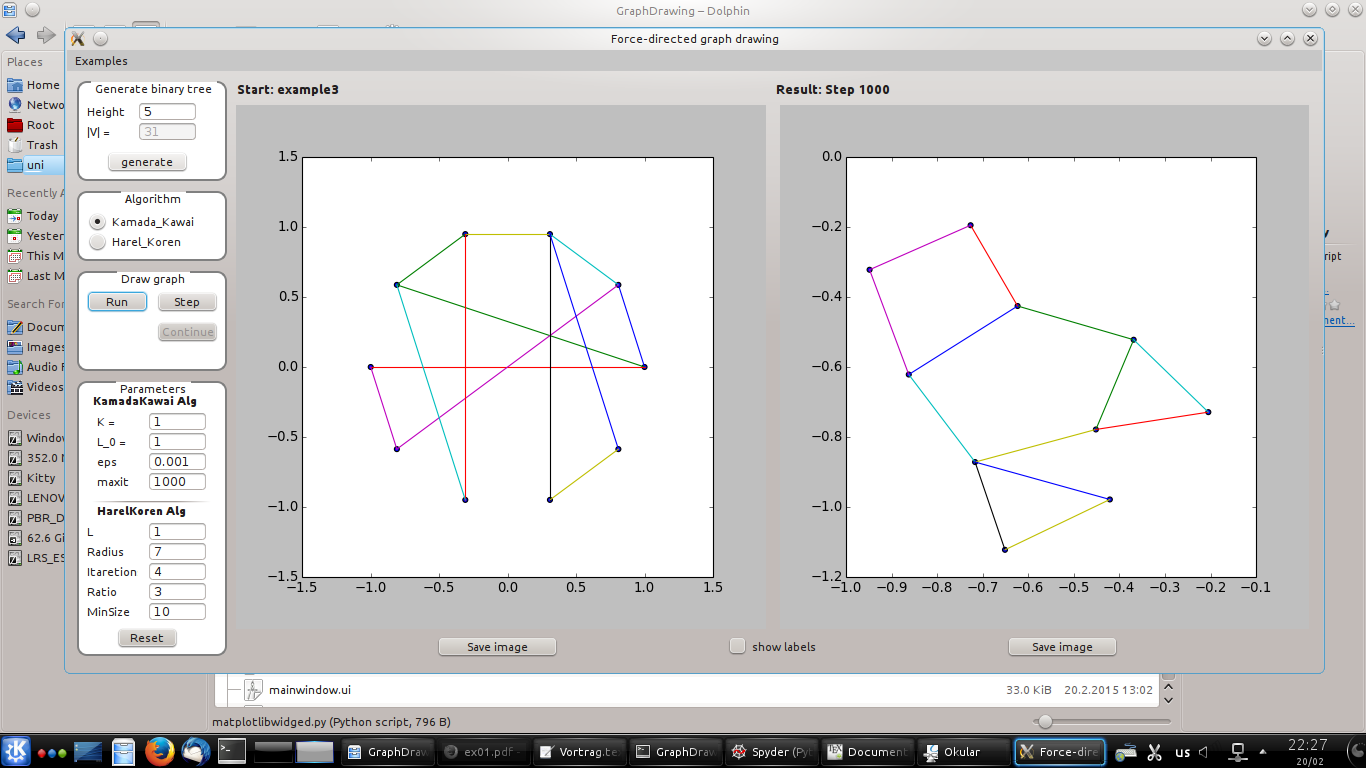
\includegraphics[scale=0.4]{interface.png}
	\caption{GUI}\label{fig: interface}
\end{figure}

In our code we used the following additional libraries : {\it numpy} (version 1.8.2), {\it matplotlib} (version 1.3.1) and {\it scipy} (version 0.13.3). Our implementation is unfortunately poorly optimized, so that better optimized versions will probably perform better. Anyway we did some optimization, as the initial implementation contained a lot of loops, which are rather slow in Python. So we used a vectorization to get rid of loops in the realisation of described the algorithms.

It is also worth mentioning that the calculation of pairwise distance between all vertices of a given graph is extremely time consuming. In our implementation we first followed the idea in \cite{TomihisaKamada1989} and used Floyd's algorithm \cite{Floyd1962} for shortest paths. Since this has complexity $ O(|V|^3)$ we also implemented a version of Dijkstras algorithm. For graphs with more than 1000 vertices we decided to use a heavily optimized version of Dijkstras algorithm from the {\it scipy} library. In both papers \cite{TomihisaKamada1989} and \cite{DavidHarel2002}, where the algorithms were presented, this problem did not arise, because the first one only considers graphs with fewer vertices and in the second paper an additional library for efficient algorithms on graphs was used.

\section{Evaluation results}

As start layout we initialize vertices of the graph uniformly on a circle with radius $L_0$ (see \cite{TomihisaKamada1989}). That means viewed as complex variables we can write 
\begin{align*}
p_m =L_0 \times e^{2 pi*i*m /n},
\end{align*}
but as it was mentioned in corresponding papers \cite{TomihisaKamada1989} and \cite{DavidHarel2002}, the initial position of the vertices has no influence on the end result, as far vertices are not placed on a single line.
Additionally, for some examples we load the initial positions of vertices from the corresponding input file (example of the 3elt graph from the collection of J.Petit \cite{JordiPetit})\\

We tested both algorithm with different graphs from \cite{TomihisaKamada1989} and \cite{DavidHarel2002}. 

\FloatBarrier 

\subsubsection*{Algorithm of Kamada and Kawai}

In fig. \ref{fig: 1} we show the initial state of a graph, the first two steps \footnote{we refer to one iteration of the outer loop as one step}  and the state the graph converges to after 49 steps. In the first step the vertex $v_2$ gets moved to the middle. In the second step the vertex $v_6$ gets moved. After this we already have a graph without edge crossing. In the following steps the movements are smaller and lead to a symmetric graph, where all the edges have the same length. \\
We also reproduced the results from fig.3 b and fig. 5 in \cite{TomihisaKamada1989} (compare fig. \ref{fig: triangGraph} and fig. \ref{fig: nonsym}). It is interesting to see, that for the non symmetric graph on Fig \ref{fig: nonsym} the algorithm did not succeed to reach the local minimum in the predefined number of iterations ($1000$). If we allow the algorithm to continue, it will only rotate the graph along its center without any changes in it's form.

In fig. \ref{fig: bincomp} we plotted the result drawings of a binary tree achieved by both algorithms. The result achieved by KKA looks slightly better. We believe that for graphs with less than $100$ vertices KKA is generally preferable.

Our performance results with KKA can be seen in table \ref{table: small}. Run time on an  Intel Core i3-2310M CPU @ 2.10GHz $\times$ 4 . Parameters were set to $K=1, \ L_0 = 1, \ \epsilon = 0.001$. % for KKA and $MinSize=10$, $Ratio=3$, $Iterations=4$, $Rad = 7$ for HKA.
We also included the results of HKA on the same graphs, which is faster, but it requires a careful setting of parameters to reach nice drawings results. We omitted the results in cases, where the applying of the HKA was not successful. 

The table also illustrates the importance of vectorisation when working in python.

\begin{table}

\begin{tabular}{|c|c||c|c|c|c|c|c|}
\hline
Algorithm: & & \multicolumn{2}{|c|}{ KKA with loops} &\multicolumn{2}{|c|}{KKA optimized} &  \multicolumn{2}{|c|}{HKA}  \\
\hline
\hline 
Graph & $|V|$ & Time & Iterations & Time & Iterations & Time & Iterations\\ 
\hline
Small Graph & 6 & 0.169s & 47& 0.05s & 53 &- & - \\ 
\hline 
Pyramid Graph & 10 & 0.370s & 45& 0.05& 46 &0.021s & 1  \\ 
\hline 
Non Symmetric Graph & 10 & FC  &FC & FC& FC & 0.024s & 1\\ 
\hline 
Binary Graph & 7 & 0.136s & 30 & 0.038s& 31 & -&-\\ 
\hline 
Binary Graph & 15 & 1.97s & 131 & 0.11s& 100 & -& - \\ 
\hline 
Binary Graph & 31 & 17.745s & 323& 0.50s & 366 & 0.032s & 1 \\ 
\hline 
\end{tabular} 
\caption[Results of KKA]{Results of KKA}
\label{table: small}
\end{table}

\FloatBarrier 

\begin{figure}[htb]
			\begin{subfigure}{.5\textwidth}
			\centering
			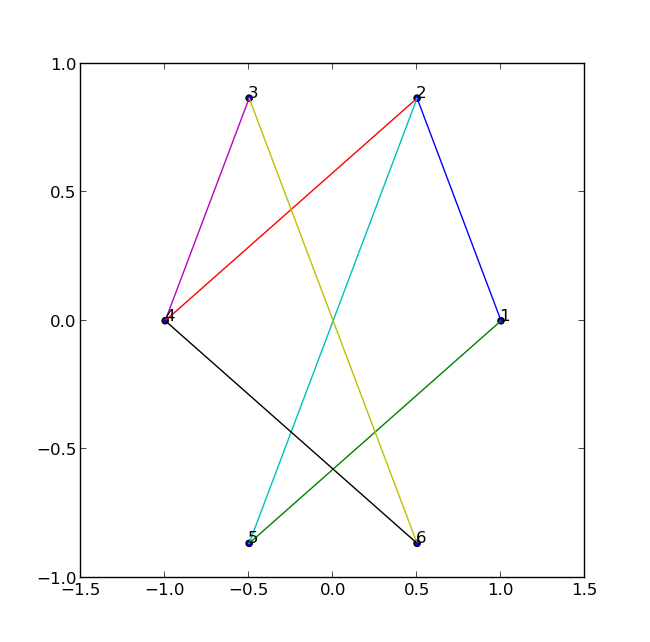
\includegraphics[scale=0.4]{results_Kawai/ex1p0}\\
			\caption{Initial State}
			\end{subfigure}\hfill
			\begin{subfigure}{.5\textwidth}
			\centering
			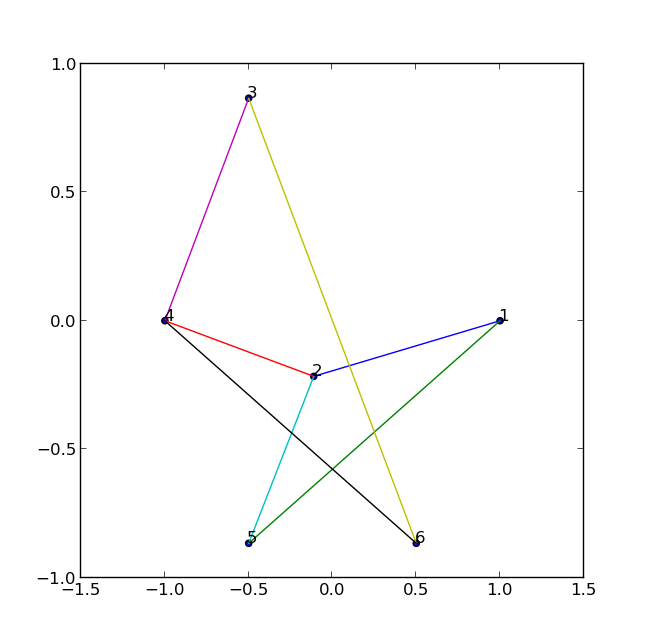
\includegraphics[scale=0.4]{results_Kawai/ex1p1}\\
			\caption{Step 1}
			\end{subfigure}
			\begin{subfigure}{.5\textwidth}
			\centering
			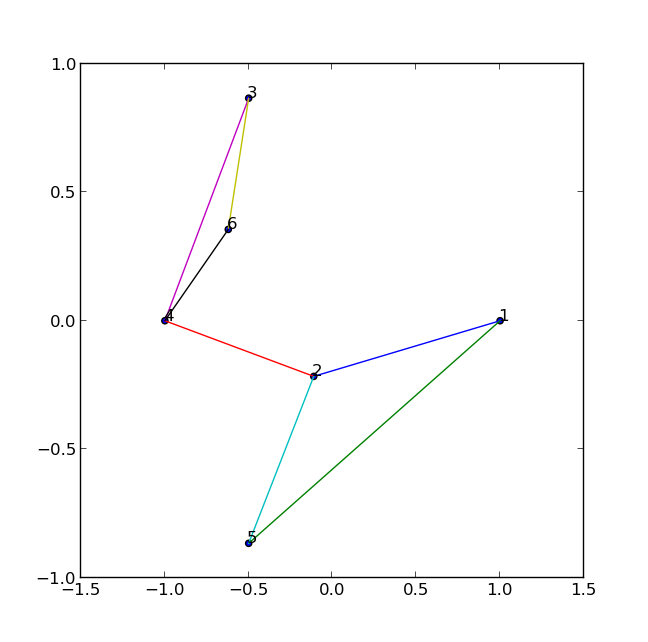
\includegraphics[scale=0.4]{results_Kawai/ex1p2}\\
			\caption{Step 2}
			\end{subfigure}\hfill
			\begin{subfigure}{.5\textwidth}
			\centering
			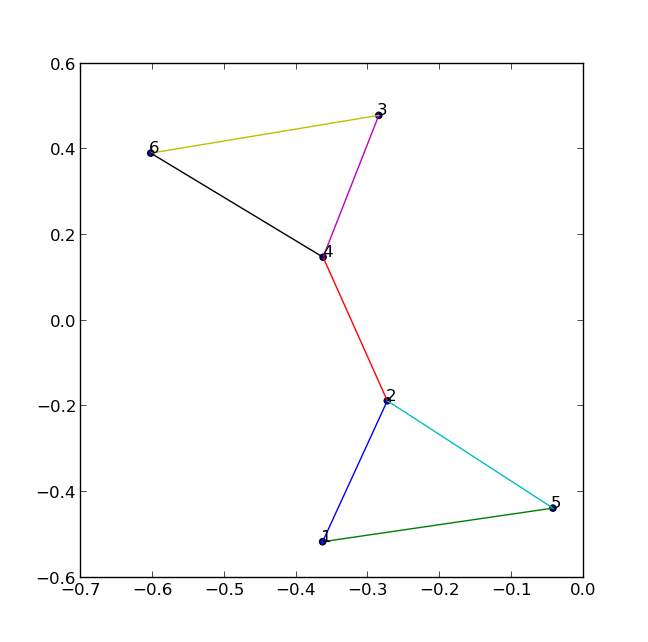
\includegraphics[scale=0.4]{results_Kawai/ex1p49}\\
			\caption{Step 49}
			\end{subfigure}\hfill

		\caption{Drawing of a small graph in 4 different states, compare fig.2 in \cite{TomihisaKamada1989}}\label{fig: 1}
\end{figure}

\begin{figure}[htb]
	 \begin{subfigure}{0.5\textwidth}
		   \centering
           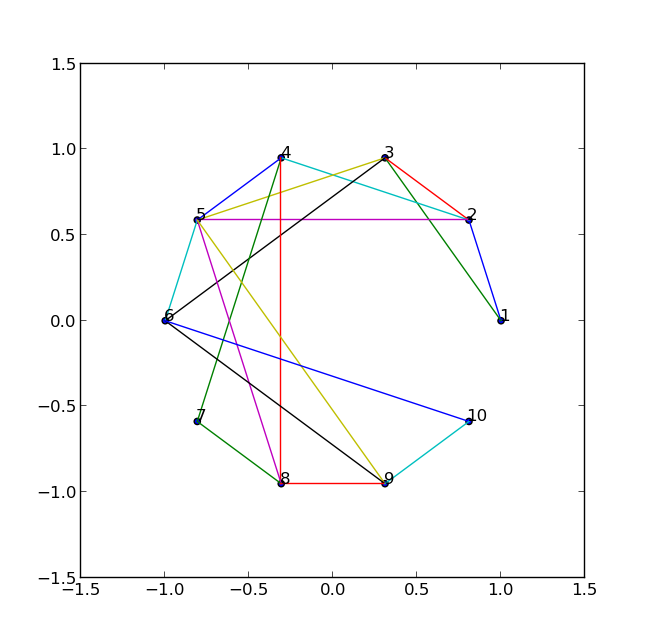
\includegraphics[scale=0.4]{results_Kawai/ex_triang_before}
           \caption{Initial State}
     \end{subfigure}
	 \begin{subfigure}{0.5\textwidth}
			\centering
           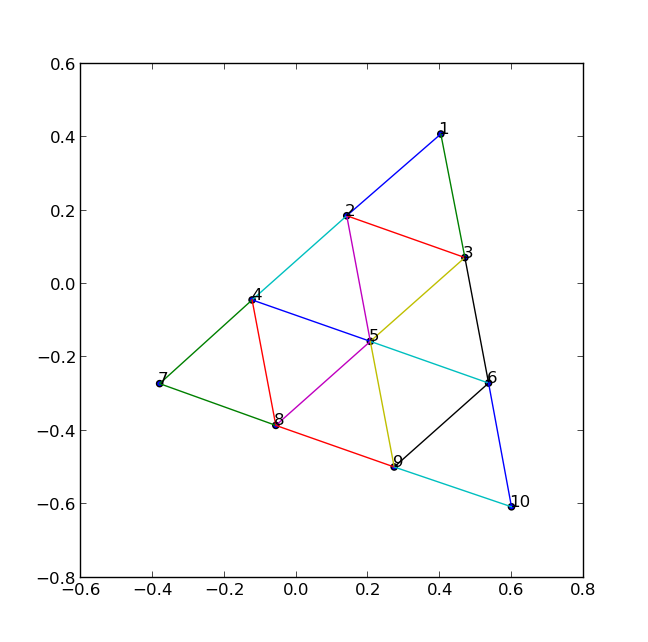
\includegraphics[scale=0.4]{results_Kawai/ex_triang_after}
            \caption{State after 46 steps}
     \end{subfigure}
     \caption{Pyramid graph (compare fig.$3 b$ in \cite{TomihisaKamada1989})}
     \label{fig: triangGraph}
\end{figure}    

\begin{figure}[htb]
	 \begin{subfigure}{0.5\textwidth}
		   \centering
           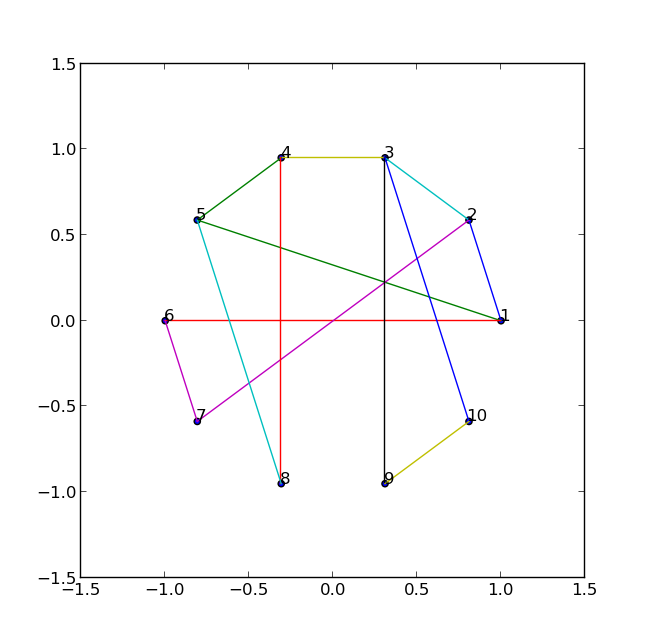
\includegraphics[scale=0.4]{results_Kawai/ex3_before}
           \caption{Initial State}
     \end{subfigure}
	 \begin{subfigure}{0.5\textwidth}
			\centering
           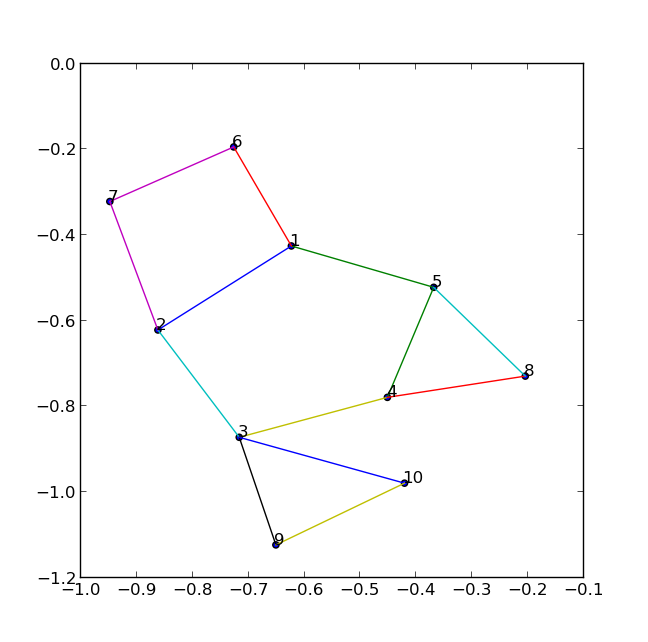
\includegraphics[scale=0.4]{results_Kawai/ex3_after}
            \caption{State after $maxit=1000$ steps}
     \end{subfigure}
     \caption{Non symmetric graph (compare fig.$5$ in \cite{TomihisaKamada1989})}
     \label{fig: nonsym}
\end{figure}    


\begin{figure}[t]
	 \begin{subfigure}{0.5\textwidth}
		   \centering
           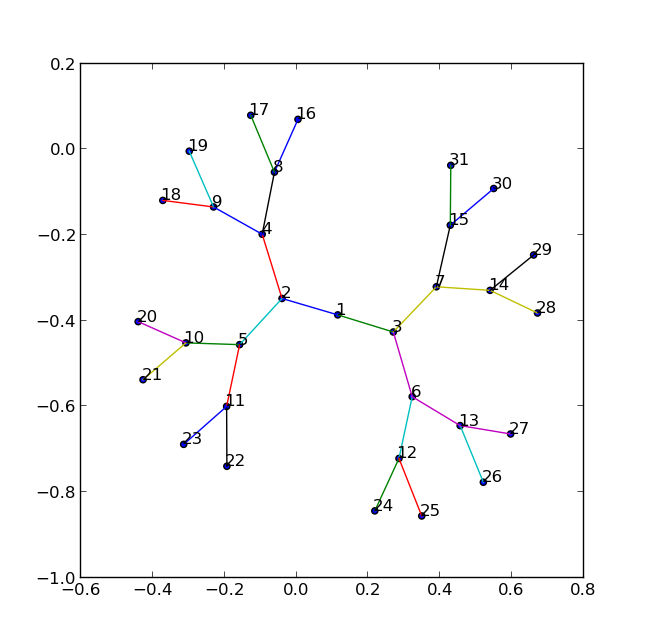
\includegraphics[scale=0.4]{results_Kawai/binary5kk}
           \caption{Result with KKA}
     \end{subfigure}
	 \begin{subfigure}{0.5\textwidth}
			\centering
           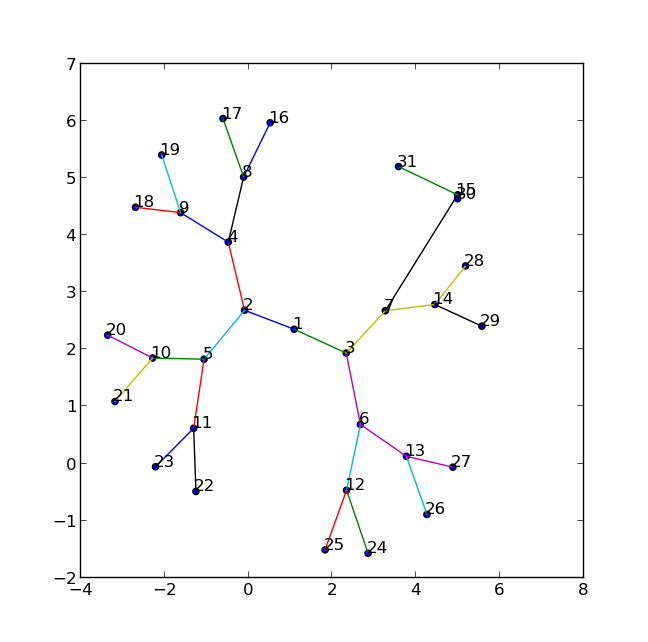
\includegraphics[scale=0.4]{results_Kawai/binary5hk}
            \caption{Result with HKA}
     \end{subfigure}
     \caption{Full Binary tree of depth $5$ for both algorithms }
     \label{fig: bincomp}
\end{figure}  


\FloatBarrier 
\subsubsection*{Algorithm of Harel and Koren}

Compared with the KKA the algorithm of Harel and Koren includes 4 parameters: minimal size of the coarsest graph ($\it MinSize$), ratio between number of vertices in two consecutive levels ($Ratio$), number of iterations of local beautification ($Iterations$), size of the neighbourhood ($Rad$). As a further parameter one can consider the desired length of graph edges ($l$), but the authors do not mention it specially. The authors claim, that for all examples in their paper they used the following parameters: $MinSize=10$, $Ratio=3$, $Iterations=4$, $Rad = 7$ (for the complete binary tree $Rad$ was set to $16$ or $17$) and achieved reasonable results.

Unfortunately, that was not always the case in our evaluation. So on figure \ref{fig: difMinSize} one can see that in case of square grid graphs some vertices stay clustered after the final iteration of the algorithm with the default settings. On the other hand, in case of complete binary tree default settings deliver better drawing results (see \ref{fig: btrees}).

\begin{figure}[htb]
	 \begin{subfigure}{0.5\textwidth}
		   \centering
           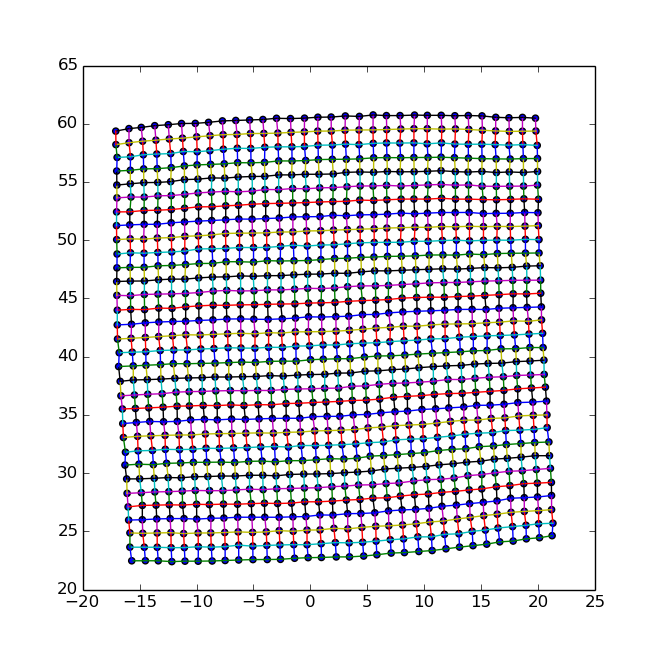
\includegraphics[scale=0.44]{results_Harel/HK_grid32x32_m2r2.png}
           \caption{$MinSize=2$, $Ratio=2$}
     \end{subfigure}
	 \begin{subfigure}{0.5\textwidth}
			\centering
           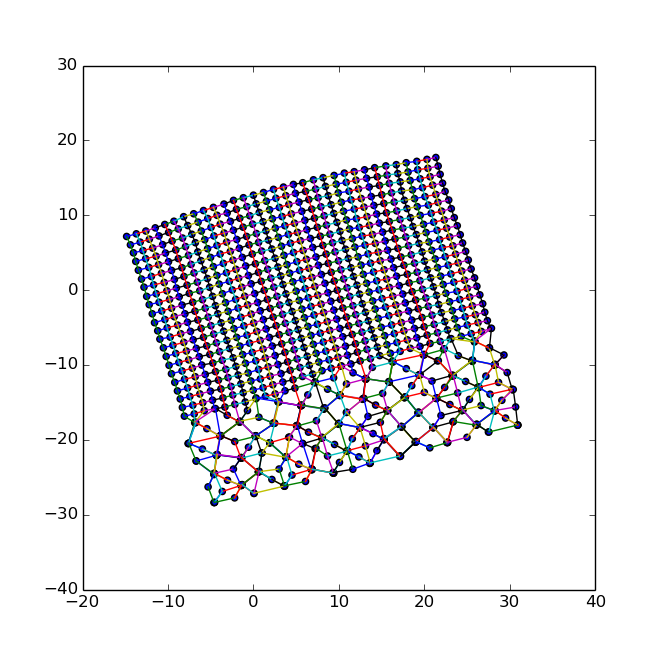
\includegraphics[scale=0.44]{results_Harel/HK_grid32x32_m10_r3.png}
            \caption{$MinSize=10$, $Ratio=3$}
     \end{subfigure}
     \caption{Square grid graph $32\times 32$ (compare fig.$1$ in \cite{DavidHarel2002})}
     \label{fig: difMinSize}
\end{figure}     

\begin{figure}[hb]
	 \begin{subfigure}{0.5\textwidth}
		   \centering
           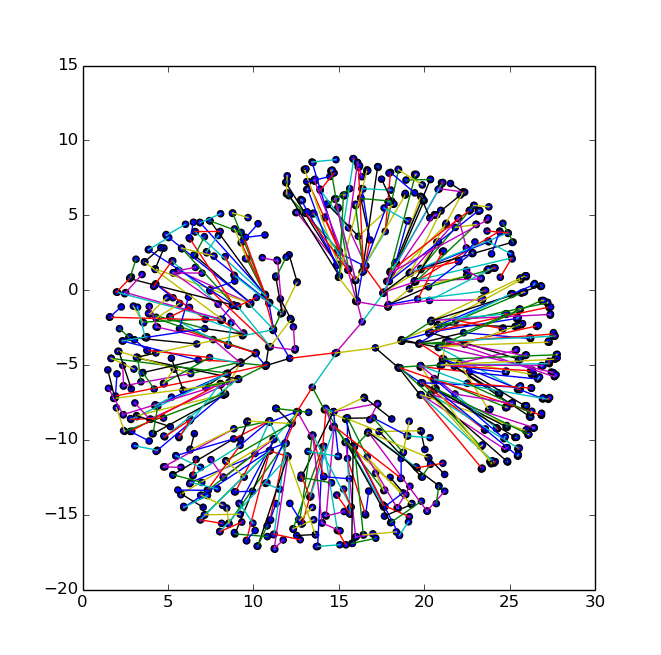
\includegraphics[scale=0.44]{results_Harel/HK_btree1023_m2_r2_rad18.png}
           \caption{$MinSize=2$, $Ratio=2$, $Rad =18$}
     \end{subfigure}
	 \begin{subfigure}{0.5\textwidth}
			\centering
           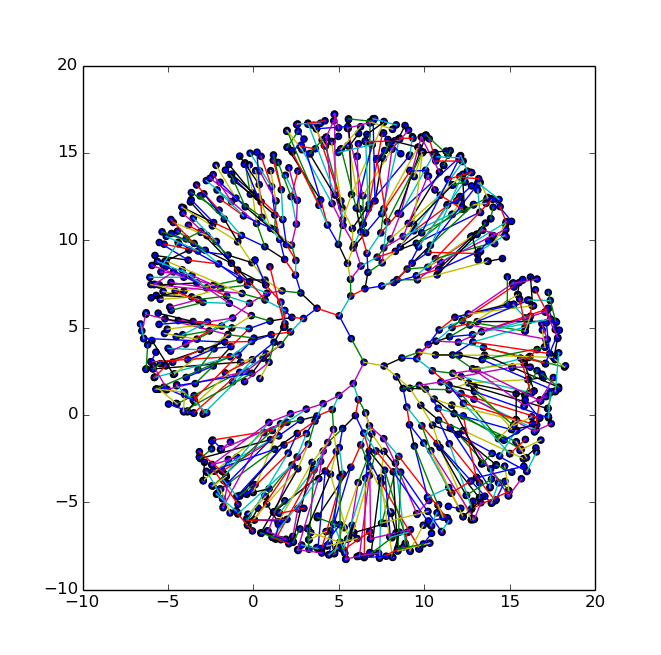
\includegraphics[scale=0.44]{results_Harel/HK_btree1023_m10_r3_rad18.png}
            \caption{$MinSize=10$, $Ratio=3$, $Rad =18$}
     \end{subfigure}
     \caption{Complete binary tree with $1023$ vertices (compare fig.$6$ in \cite{DavidHarel2002})}
     \label{fig: btrees}
\end{figure}     

\FloatBarrier 

We also found out, that a random noise added to vertex coordinates (see line $10$ in algorithm \ref{HK}) has some impact on the end result. On fig. \ref{fig: compareRand} one can see that adding smaller noise (for example from $(0,0)$ to $(0.1, 0.1)$) leads to better drawing result in our implementation. Convinced by this result, we added factor $0.1$ to $rand$ in original algorithm.

\begin{figure} [htb]
\begin{minipage}[0.2\textheight]{\textwidth}	%step3
	 \begin{subfigure}{0.5\textwidth}
		   \centering
           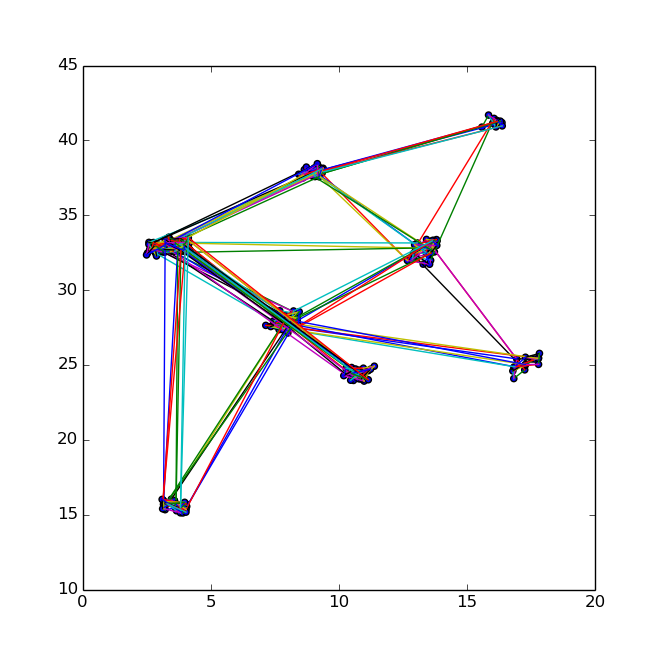
\includegraphics[scale=0.3]{results_Harel/rand1/HK_step3_eps1.png}
           \caption{Step $3$}
     \end{subfigure}
	 \begin{subfigure}{0.5\textwidth}
			\centering
            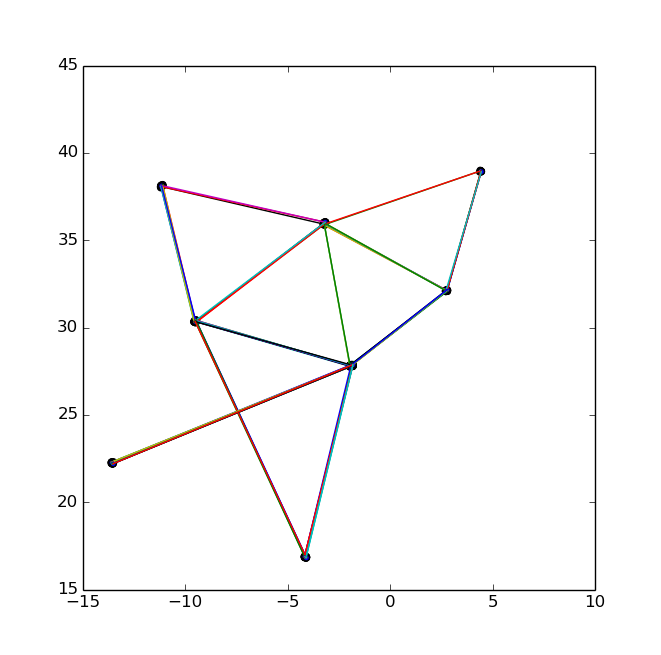
\includegraphics[scale=0.3]{results_Harel/rand01/HK_step3_eps01.png}
            \caption{Step $3$}
     \end{subfigure}        
\end{minipage}

\begin{minipage}[0.2\textheight]{\textwidth}	%step5
	 \begin{subfigure}{0.5\textwidth}
		   \centering
           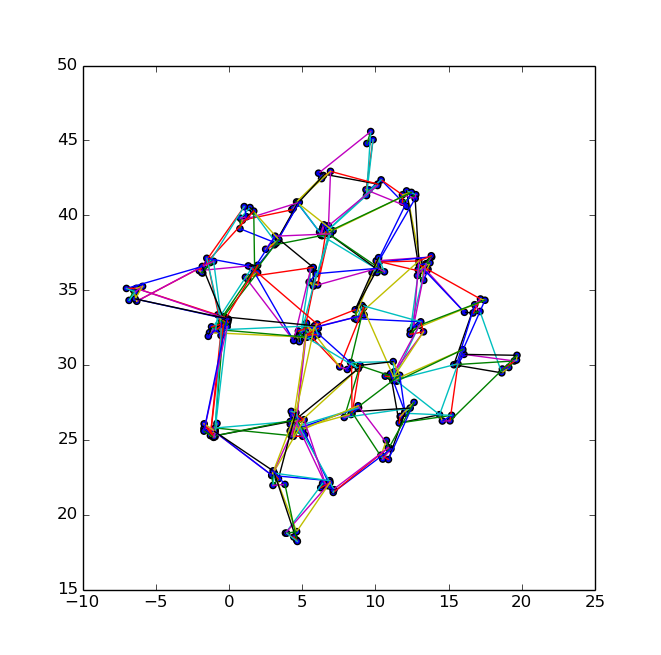
\includegraphics[scale=0.3]{results_Harel/rand1/HK_step5_eps1.png}
           \caption{Step $5$}
     \end{subfigure}
	 \begin{subfigure}{0.5\textwidth}
	 			\centering
            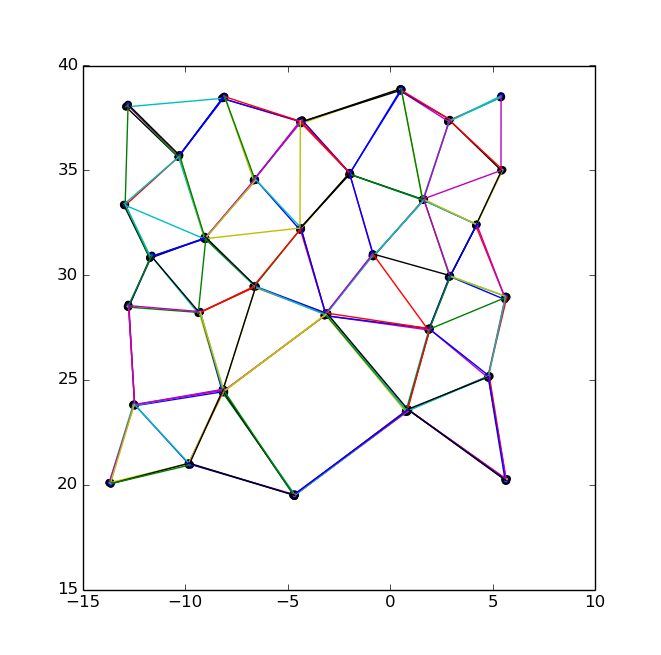
\includegraphics[scale=0.3]{results_Harel/rand01/HK_step5_eps01.png}
            \caption{Step $5$}
     \end{subfigure}        
\end{minipage}
\begin{minipage}[0.2\textheight]{\textwidth}	%step8
	 \begin{subfigure}{0.5\textwidth}
		   \centering
           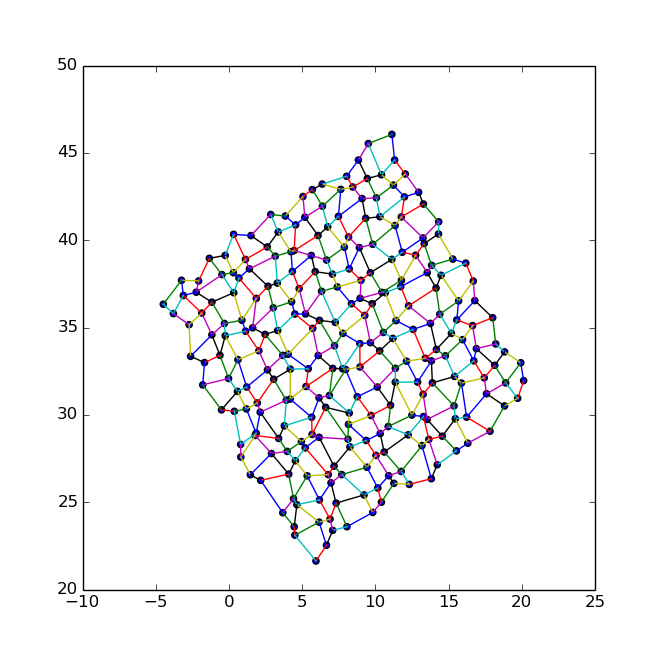
\includegraphics[scale=0.3]{results_Harel/rand1/HK_step8_eps1.png}
           \caption{Step $8$}
     \end{subfigure}
	 \begin{subfigure}{0.5\textwidth}
	 	    \centering
            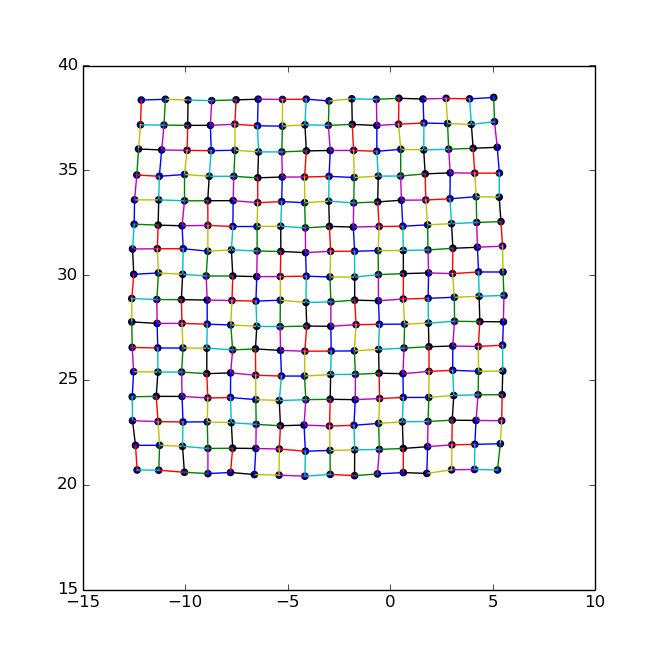
\includegraphics[scale=0.3]{results_Harel/rand01/HK_step8_eps01.png}
            \caption{Step $8$}
     \end{subfigure}        
\end{minipage}

\caption{Influence of the random noise HKA on the example of grid graph $16\times16$. Left column : $(0,0)<rand<(1,1)$, right column - $(0,0)<rand<(0.1,0.1)$}
\label{fig: compareRand}
\end{figure}	

\FloatBarrier

In figure \ref{fig: sgrid} we show the result of applying the HKA to the sparse grid graphs ($1/3$ of edges were omitted). Unfortunately, the images do not look so spectacular as in the original paper (see fig.$4$ in \cite{DavidHarel2002}).
\begin{figure}[htb]
	 \begin{subfigure}{0.5\textwidth}
		   \centering
           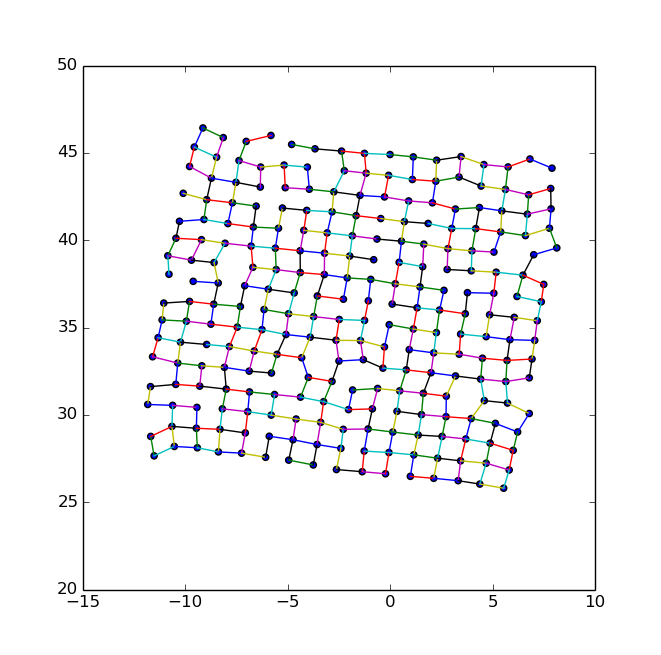
\includegraphics[scale=0.45]{results_Harel/HK_sgrid16x16_m2r2.png}
           \caption{Sparse square grid graph $16\times 16$ ($256$ vertices), $MinSize=2$, $Ratio=2$}
     \end{subfigure}
	 \begin{subfigure}{0.5\textwidth}
			\centering
           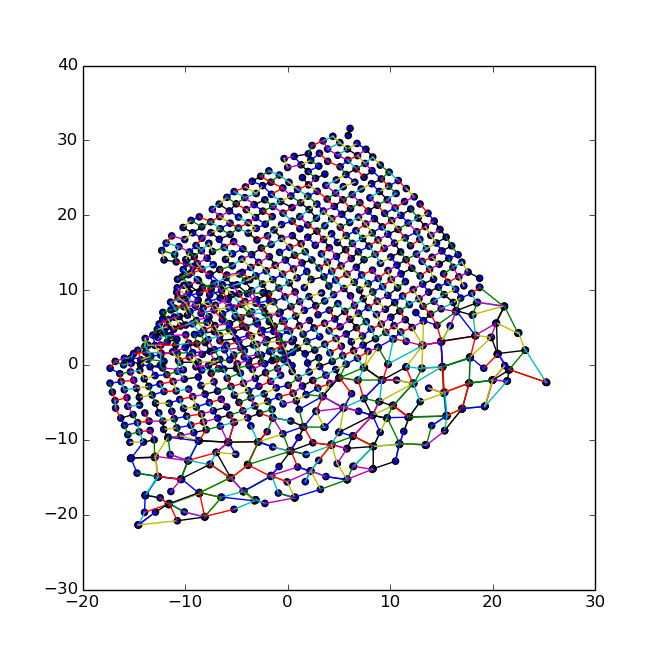
\includegraphics[scale=0.45]{results_Harel/HK_sgrid32x32_m10_r3.png}
            \caption{Sparse square grid graph $32\times 32$ ($1024$ vertices), $MinSize=10$, $Ratio=3$}
     \end{subfigure}
     \caption{Sparse square grid graphs (compare fig.$4$ in \cite{DavidHarel2002}}
     \label{fig: sgrid}
\end{figure}     

\newpage

The performance of our implementation of HKA can be seen in table \ref{table: large}. Computations were made on an Intel Core i7-3520M CPU @ 2.90GHz$\times 4$.

%\begin{table}[htb]
%\small
%\begin{tabular}{|c|c||c|c|c|c|c|}
%\hline
%Algorithm: & & \multicolumn{2}{|c|}{Kamada Kawai} &  \multicolumn{2}{|c|}{Multi Scale} & Parameters \\
%\hline
%\hline 
%Complete Binary Graph & 255  & & & $0.626503$s    & $3$ & $MinSize=10$, $Ratio=3$, $Rad = 18$\\ 
%\hline 
%Complete Binary Graph & 1023 & & & $1402.674150$s & $5$ & $MinSize=10$, $Ratio=3$,$Rad = 18$\\ 
%\hline 
%Complete Binary Graph & 1023 & & & $??????$s & $9$ & $MinSize=2$, $Ratio=2$, $Rad = 18$\\ 
%\hline \hline
%Square Grid Graph     & 256 & & & $20.029714$s & $8$ & $MinSize=2$, $Ratio=2$\\ 
%\hline
%Square Grid Graph     & 256 & & & $0.615102$s & $3$ & $MinSize=10$, $Ratio=3$\\ 
%\hline
%Square Grid Graph     & 1024 & & & $3854.181407$s & $10$ & $MinSize=2$, $Ratio=2$\\ 
%\hline
%Square Grid Graph     & 1024 & & & $1403.437832$s & $5$ & $MinSize=10$, $Ratio=3$\\ 
%\hline\hline
%Sparse Square Grid Graph & 256 & & & $20.168194$s & $8$ & $MinSize=2$, $Ratio=2$\\ 
%\hline
%Sparse Square Grid Graph & 1024 & & & $1439.099359$s & $5$ & $MinSize=10$, $Ratio=3$\\ 
%\hline 
%\end{tabular} 
%\caption{Results for large graphs}
%\label{table: large}
%\end{table}

\begin{table}[htb]
\small
\begin{tabular}{|c|c||c|c|c|c|c|}
\hline
Algorithm HKA & $|V|$ & Parameters & \multicolumn{2}{|c|}{HKA} \\
\hline
\hline 
Complete Binary Graph & 255 & $MinSize=10$, $Ratio=3$, $Rad = 18$ & $0.626503$s    & $3$ \\ 
\hline 
Complete Binary Graph & 1023 & $MinSize=10$, $Ratio=3$,$Rad = 18$ & $1402.674150$s & $5$ \\ 
\hline 
Complete Binary Graph & 1023 & $MinSize=2$, $Ratio=2$, $Rad = 18$ & $261.274154$s & $9$ \\ 
\hline \hline
Square Grid Graph     & 256 & $MinSize=2$, $Ratio=2$ & $20.029714$s & $8$ \\ 
\hline
Square Grid Graph     & 256 & $MinSize=10$, $Ratio=3$& $0.615102$s & $3$ \\ 
\hline
Square Grid Graph     & 1024 & $MinSize=2$, $Ratio=2$ & $3854.181407$s & $10$ \\ 
\hline
Square Grid Graph     & 1024 & $MinSize=10$, $Ratio=3$ & $1403.437832$s & $5$ \\ 
\hline\hline
Sparse Square Grid Graph & 256 & $MinSize=2$, $Ratio=2$ & $20.168194$s & $8$ \\ 
\hline
Sparse Square Grid Graph & 1024 & $MinSize=10$, $Ratio=3$ & $1439.099359$s & $5$ \\ 
\hline 

\end{tabular} 
\caption{Results of HKA (optimized version) for large graphs}
\label{table: large}
\end{table}

\FloatBarrier 

As we have alredy mentioned, our first implementation consisted of many loops. For example, before using verctorization the time needed to draw the complete binary three with $1023$ vertices counted $30527.096519$s comparing to $1402.674150$s or $261.274154$s after optimization.

\section{Conclusions}

%We successfully implemented the algorithms described in \cite{TomihisaKamada1989} and \cite{DavidHarel2002} and were able to replicate most of %their results. We found out that KKA is a good choice for drawing small graphs but takes too long for a high number of vertices. HKA is much %better suited for handling larger graphs. But it also has the problem that we need to compute and store the complete distance matrix $d$, %which is expensive. Hence, we encountered difficulties with the graphs that had more than $1024$ vertices. If we were to keep working on the %graph drawing problem we see two possibilities. We could try to further optimize our implementation of HKA. However we might need to port it %in a language like C++ to achieve the speed described in \cite{DavidHarel2002}. The more interesting thing to do would be to follow another %idea by Harel and Koren and take a look at \cite{Harel2004}. Here the authors propose a new approach where they first embed the graph in a %high dimensional space and then project it into 2D using principal component analysis. This would lead us back to the theory we encountered in %our Machine Learning lecture.  

We successfully implemented the algorithms described in \cite{TomihisaKamada1989} and \cite{DavidHarel2002} and were able to reproduce most of their results. 

We found out that KKA is a good choice for drawing small graphs but takes too long for a high number of vertices.

HKA is much better suited for handling larger graphs. Unfortunately, in our implementation the HKA is not so fast, as it is mentioned in the paper. So we were not able to test it on the graphs with more then $1024$ vertices in reasonable time. Also, using the same parameters for all graph types, as it was made in the paper \cite{DavidHarel2002}, did not lead in our case to the equally good results for all graphs. On the other hand, changing the parameters to get better results led to increased running time. \\
As we already have mentioned, our implementation could be better optimized. If we were to keep working on the graph drawing problem we see two possibilities. We could try to further optimize our implementation of HKA. However we might need to port it in $C++$ to achieve the same speed described in \cite{DavidHarel2002}. There the algorithm was initially implemeted in $C++$ using an additional library for efficient graph algorithms.

The more interesting thing to do would be to follow another idea by Harel and Koren and take a look at \cite{Harel2004}. Here the authors propose a new approach where they first embed the graph in a high dimensional space and then project it into 2D using principal component analysis. This would lead us back to the theory we encountered in our Machine Learning lecture.

\vspace{30pt}

The impact on the implementation was divided uniquelly between the authors. The KKA was implemented and tested by Mr. Roeger, the HKA as well as the GUI by Mrs.Tikhoncheva. Additional functions such as reading the adjacency matrix and coordinates of the vertices from a file, generating of complete binary trees, floyd algorithm were implemented by Mr. Roeger.

After the first performance tests we encountered that the performance was rather poor. Therefore after discussion on the possible improvement the matrix approach suggested by Mr. Roeger was implemented by Mrs. Tikhoncheva.



\bibliography{literatur}
\bibliographystyle{siam}

\end{document}